\chapter{Evaluation}
\label{chap:evaluation}

\glsreset{mae}
\glsreset{mse}
\glsreset{rmse}
\glsreset{r2}
% \glsresetall

This chapter thoroughly evaluates our generalization strategy by comparing the three model variants proposed in section \ref{sec:model-variants}.



\section{Methodologies}
\label{sec:evaluation-methods}

The comparison includes both quantitative and qualitative evaluations. On one side, a quantitative valuation provides numerical results, which are crucial for scientifically assessing the network's capabilities through a set of chosen metrics. On the other side, qualitative observations rely on human interpretation to evaluate models' possible behaviors in some real contexts.

The first part of this chapter focuses on the application of statistical metrics for quantitatively examine the three models both on the training (section \ref{sec:evaluation-training}) and the test set (section \ref{sec:evaluation-quantitative}). The former is used to briefly understand overall models' learning, while the latter aims to submit unseen examples for assessing the networks' capability in generalization.

An official test set is made available by Mantegazza et al. \cite{mantegazza2019visionbased}. For enhancing testing capabilities, we take advantage of background replacement to generate artificial datasets from the test set. Even though this technique can lead to potential biases during the evaluation, caused by unrealistic patterns possibly created during the image manipulation, it allows performing quantitative evaluations without the need of recording new data in different environments.

\subsubsection*{Metrics}

Qualitative evaluation mostly concerns direct comparisons between the models' predictions and the ground truth. On the contrary, quantitative results require statistical computations suited for regression, thus commonly used in machine learning. The following list presents an overview of all the principal metrics adopted for our evaluation and used in the next sections.

\begin{itemize}
    \item \gls{mae} measures the average residuals in the dataset, which means the absolute difference between the actual and predicted values. The lower the \gls{mae}, the better the model. Considering $y_i$ the predicted value and $\hat{y_i}$ the actual value:
    $$ MAE = \frac{1}{N} \sum_{i=1}^N |y_i - \hat{y_i}| $$
    
    \item \gls{rmse} measures the standard deviation of residuals. As for \gls{mae}, \gls{rmse} should be as lower as possible. It penalizes large prediction errors, thus is not particularly suited to be used on a dataset with many outliers. The main advantage and reason for its usage in evaluating regression models is because \gls{rmse} has the same unit as the dependent variable, so it is easy to interpret.
    $$ RMSE = \sqrt{\frac{1}{N} \sum_{i=1}^N (y_i - \hat{y_i})^2} $$
    
    \item \gls{r2} (or coefficient of determination) measures the robustness of the regression. It represents the proportion of the variance in the dependent variable which is explained by the independent variable. As such variance is dataset dependent, \gls{r2} may not be meaningfully comparable across different datasets. Thus, the metric should only be compared among different models for the same dataset but not on different datasets for the same model.
    
    \gls{r2} is often the best choice for evaluating regression performance because it provides a measure of fitness for the model to predict unseen data correctly. Also, its domain is easily understandable since it goes from $-\infty$ to 1: an optimal model (with no prediction errors) will have an \gls{r2} of 1; a model that always predicts the average value will have an \gls{r2} of 0; a model worse than the average predictor will have a negative \gls{r2}. Considering $\overline{y}$ the mean value:
    $$ R^2 = 1 - \frac{\sum_{i=1}^N (y_i - \hat{y_i})^2}{\sum_{i=1}^N (y_i - \overline{y})^2} $$
\end{itemize}




\section{Training Results}
\label{sec:evaluation-training}

As for the entire chapter, this section considers the \texttt{Arena}, \texttt{CVPR} and \texttt{CVPR Aug} models defined in section \ref{sec:model-variants}. Here, we introduce their performance during the training procedure presented in section \ref{sec:implementation-training}.

In this phase, the loss function (\gls{mae}) and the \gls{r2} score are take into consideration, both for the train and the validation set. Figures \ref{fig:training-metrics-arena}, \ref{fig:training-metrics-cvpr} and \ref{fig:training-metrics-cvpraug} show metrics evolution over the 60 training epochs. Overall, it can be said that at least 30 epochs are needed to reach the convergence, after which the performance stabilizes.

\texttt{Arena}, \texttt{CVPR}, and \texttt{CVPR Aug} achieve a validation loss of 0.07, 0.13 and 0.20, respectively. As the model complexity increases, the loss does; however, the gap between training and validation loss decreases, as shown in the figure. This may be a symptom of better generalization capabilities, although we do not yet have enough information to draw a conclusion on the subject. Even though the \texttt{CVPR Aug} model appears to be able to improve by further increasing the number of epochs, experiments with 200 epochs have substantially the same results as 60.

The \texttt{Arena} model registers an \gls{r2} of 0.99, which can be attributable to overfitting. In fact, such a score would be obtained by an optimal model, but we already know that the original FrontalNet by \cite{mantegazza2019visionbased} could not properly work outside of the drone arena. In the next sections, we will examine models \texttt{CVPR} and \texttt{CVPR Aug} on various test sets to certify their robustness against the \texttt{Arena} one.

\begin{figure}[H]
	\centering
	\includegraphics[width=1 \textwidth]{"contents/images/06-training-arena"}
	\caption[\texttt{Arena} model's performance during training. Loss and \gls{r2} on training and validation sets]{\texttt{Arena} model's performance during training. Loss and \gls{r2} on training and validation sets}
	\label{fig:training-metrics-arena}
\end{figure}

\begin{figure}[H]
	\centering
	\includegraphics[width=1 \textwidth]{"contents/images/06-training-CVPR"}
	\caption[\texttt{CVPR} model's performance during training. Loss and \gls{r2} on training and validation sets]{\texttt{CVPR} model's performance during training. Loss and \gls{r2} on training and validation sets}
	\label{fig:training-metrics-cvpr}
\end{figure}

\begin{figure}[H]
	\centering
	\includegraphics[width=1 \textwidth]{"contents/images/06-training-CVPRaug"}
	\caption[\texttt{CVPR Aug} model's performance during training. Loss and \gls{r2} on training and validation sets]{\texttt{CVPR Aug} model's performance during training. Loss and \gls{r2} on training and validation sets}
	\label{fig:training-metrics-cvpraug}
\end{figure}




\section{Quantitative Evaluation}
\label{sec:evaluation-quantitative}

\lipsum[1-2]

loss, r2, and rmse comparison over the 3 models and 3 test sets

As described before, \gls{r2} represents the proportion of variance in the dependant variable (the target) that has been explained by the independent variables in the model (the features). As such variance is dataset dependent, \gls{r2} may not be meaningfully comparable across different datasets. Thus, the metric should can only be compared among different models for the same dataset, but not on different datasets for the same model.

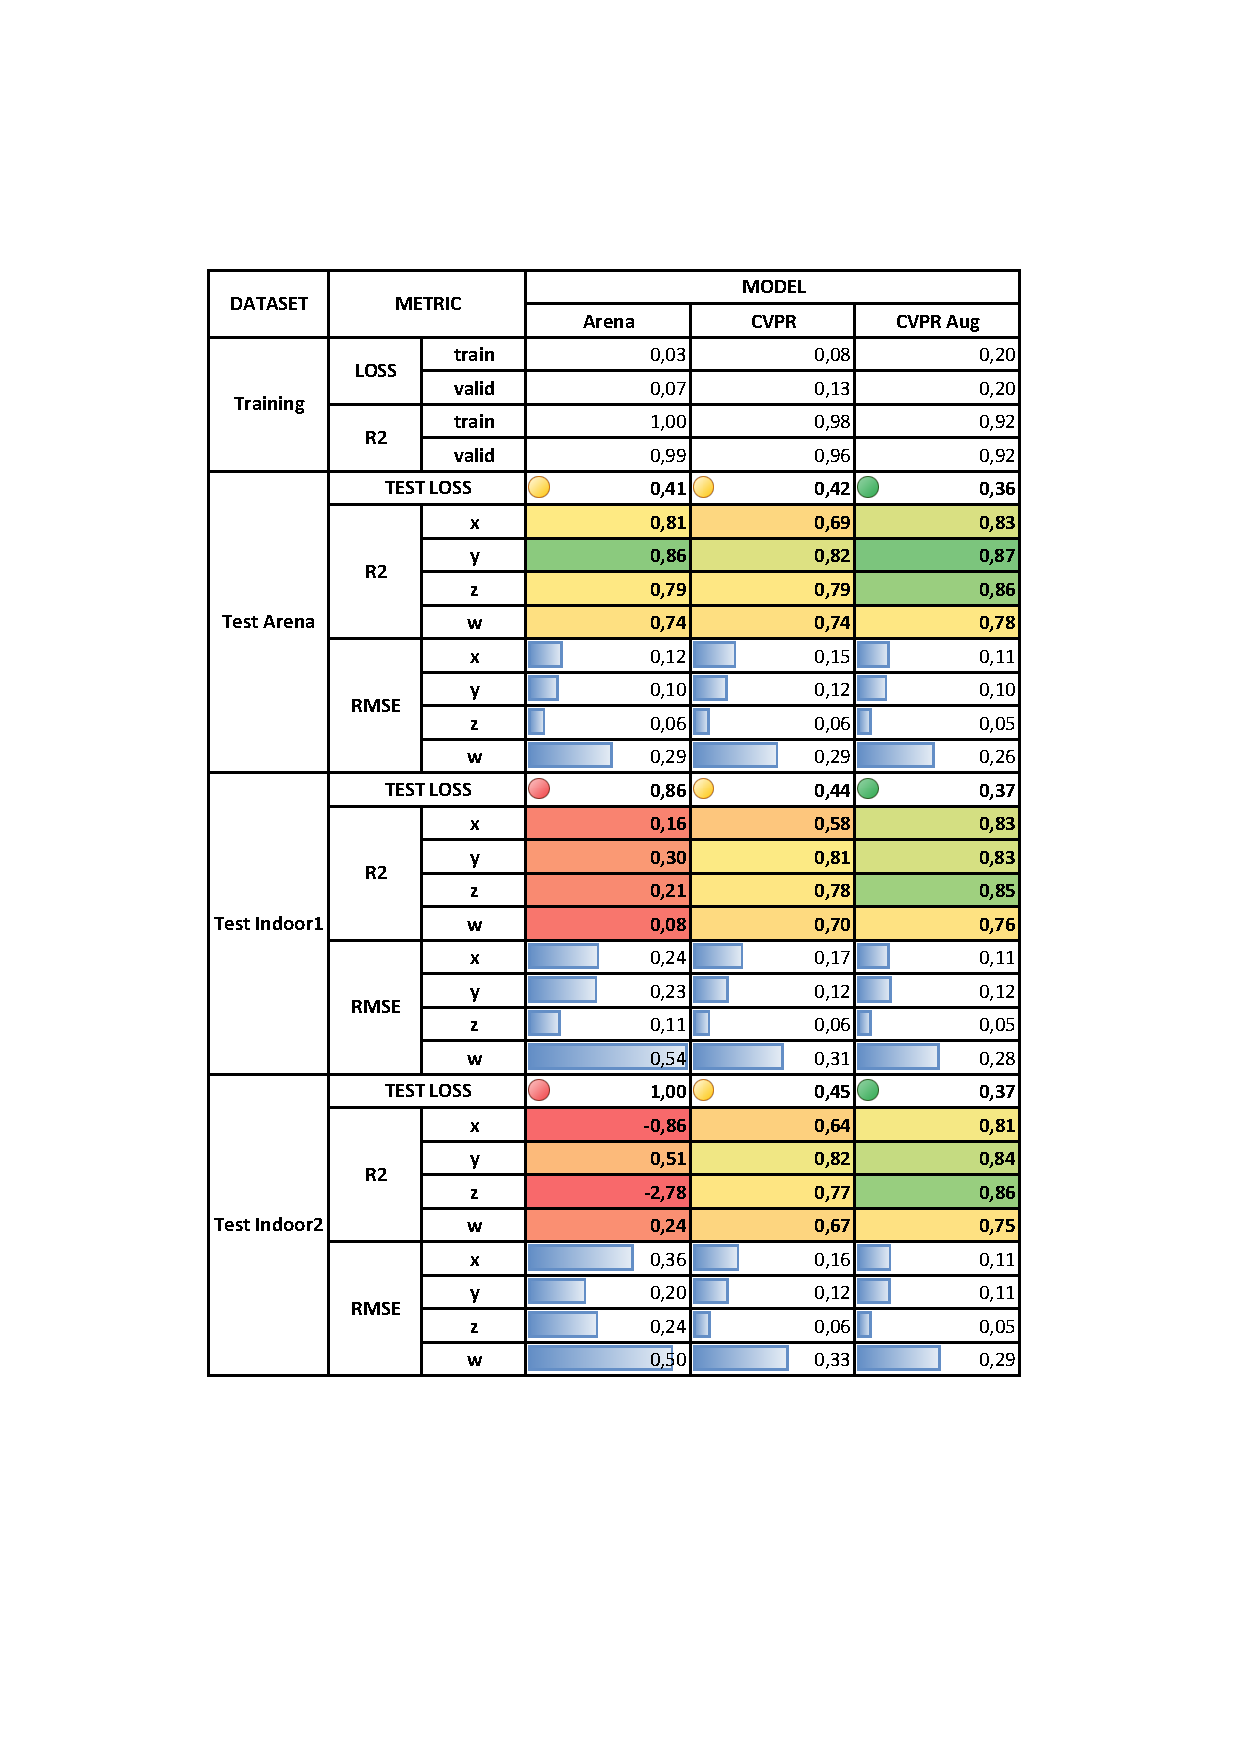
\includepdf[pages={1}]{contents/images/06-qt-summary}


\section{Qualitative Evaluation}
\label{sec:evaluation-qualitative}

Charts: video frames with predictions comparison; time series GT \& pred \textbf{model} comparison; time series GT \& pred \textbf{background} comparison for a given model; variance considerations

- arena dataset

- bg replaced dataset

- phone videos dataset


\section{Summary}
\label{sec:evaluation-summary}

conclusions